% TODO famous example for a product line failure?

\subsection{Recap: Software Testing}
\begin{frame}{\myframetitle}
	\begin{mycolumns}
		\uncover<1->{\mydefinition{Software Testing \mysource{\sommerville}}{\mycite{Testing is intended to show that a program does what it is intended to do and to discover program defects before it is put into use.}}{}}
		\uncover<2->{\mydefinition{Validation Testing \mysource{\sommerville}}{\mycite{Demonstrate to the developer and the customer that the software meets its requirements.}}{}}
		\uncover<3->{\mydefinition{Defect Testing \mysource{\sommerville}}{\mycite{Find inputs or input sequences where the behavior of the software is incorrect, undesirable, or does not conform to its specification.}}{}}
	\mynextcolumn
		\uncover<4->{\mynote{Stages of Testing \mysource{\sommerville}}{
			\begin{itemize}
				\setlength\itemsep{.1em}
				\item[1.] \mycite{\emph{Development testing}, where the system is tested during development to discover
				bugs and defects}
				\item[2.] \mycite{\emph{Release testing}, where a separate testing team tests a complete version of the
				system before it is released to users}
				\item[3.] \mycite{\emph{User testing}, where users or potential users of a system test the system in their
				own environment}
			\end{itemize}
		}}
		\uncover<5->{\mynote{Manual vs Automated Testing \mysource{\sommerville}}{\mycite{In \emph{manual testing}, a tester runs the program with some test data and
				compares the results to their expectations. [...] In \emph{automated testing}, the tests are encoded in a program that is run each time the system under development is to be tested.}}}
	\end{mycolumns}
\end{frame}

% TODO recap analysis strategies for product lines and discuss why feature based and family based is typically not feasible for testing

\subsection{Testing All Configurations}
\begin{frame}{\myframetitle}
	\leftorright{
		\centering\featureDiagramConfigurableDatabase
		
		\begin{example}{Recap: 26 Valid Configurations\mysource{\lecturemodeling}}
			\footnotesize
			\begin{mycolumns}[animation=none]
				$\{C,G,W\}$\\
				$\{C,P,W\}$\\
				$\{C,G,P,W\}$\\
				$\{C,D,W\}$\\
				$\{C,G,D,W\}$\\
				$\{C,P,D,W\}$\\
				$\{C,G,P,D,W\}$\\
				$\{C,P,T,W\}$\\
				$\{C,G,P,T,W\}$\\
				$\{C,D,T,W\}$\\
				$\{C,G,D,T,W\}$\\
				$\{C,P,D,T,W\}$\\
				$\{C,G,P,D,T,W\}$
			\mynextcolumn
				$\{C,G,L\}$\\
				$\{C,P,L\}$\\
				$\{C,G,P,L\}$\\
				$\{C,D,L\}$\\
				$\{C,G,D,L\}$\\
				$\{C,P,D,L\}$\\
				$\{C,G,P,D,L\}$\\
				$\{C,P,T,L\}$\\
				$\{C,G,P,T,L\}$\\
				$\{C,D,T,L\}$\\
				$\{C,G,D,T,L\}$\\
				$\{C,P,D,T,L\}$\\
				$\{C,G,P,D,T,L\}$
			\end{mycolumns}
		\end{example}
	}{
		\vspace{-7mm}
		\mynote{Discussion}{
			\begin{itemize}
				\setlength\itemsep{.5em}
				\item only feasible for small product lines (few valid configurations)
				\item redundant test effort
				\item large product lines: not even feasible to generate and compile all configurations
				\item (some) large product lines: not even the number of valid configurations is known
			\end{itemize}
		}
	}
\end{frame}

\begin{frame}{Recap: Feature Model of the Linux Kernel}
	\vspace{28mm}~\hspace{-15mm}\href{https://dl.acm.org/doi/abs/10.1145/3382025.3414943}{\includegraphics[width=1.2\linewidth,page=1,trim=100 510 100 170,clip]{2020/2020-SPLC-Thuem}}
\end{frame}

\begin{frame}{\myframetitle}
	\begin{mycolumns}[widths={60}]
		\myexampletight{Recap: Industrial Configuration Spaces\mysource{\lectureintroduction}}{
			\centering\evaluatingsharpsatsolverslink{\includegraphics[width=\linewidth,page=6,trim=50 210 320 440,clip]{2020/2020-VaMoS-Sundermann}}
		}
		\uncover<3->{\mynote{}{Why being complete on the configurations then?}}
	\mynextcolumn
		\href{https://commons.wikimedia.org/wiki/File:Edsger_Wybe_Dijkstra.jpg}{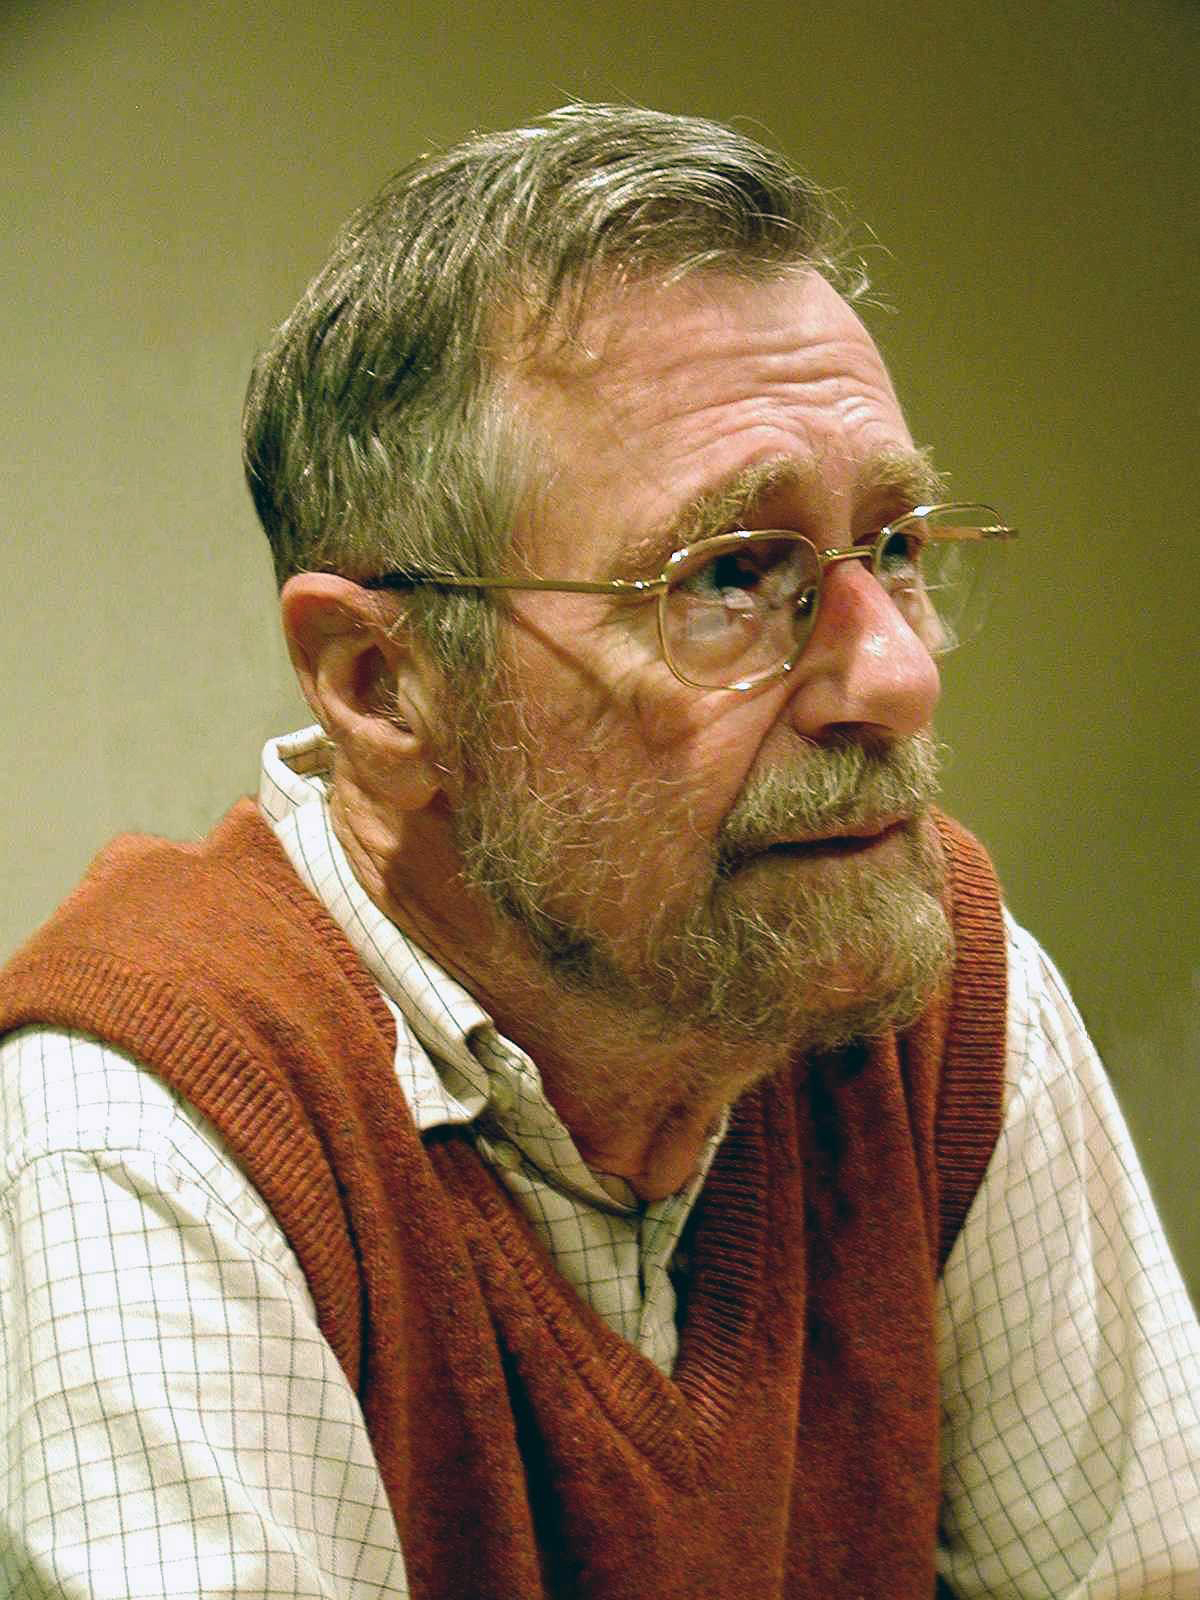
\includegraphics[width=\linewidth,trim=0 425 0 75,clip]{edsger-dijkstra}}
		\vspace{-7mm}
		
		\mynote{Edsger W. Dijkstra (1972)}{\mycite{Program testing can be a very effective way to show the presence of bugs, but it is hopelessly inadequate for showing their absence.}\mysource{\thehumbleprogrammer}}
		% 1930-2002, ACM Turing Award winner
	\end{mycolumns}
\end{frame}

\newcommand{\eemph}[1]{{\color{red}\textbf{#1}}}

\subsection{Testing One Configuration}
\begin{frame}[b]{\myframetitle}
	\begin{mycolumns}[b]
		\centering\featureDiagramConfigurableDatabase
		
		\begin{example}{Recap: 26 Valid Configurations\mysource{\lecturemodeling}}
			\footnotesize
			\leftandright{
				$\{C,G,W\}$\\
				$\{C,P,W\}$\\
				$\{C,G,P,W\}$\\
				$\{C,D,W\}$\\
				$\{C,G,D,W\}$\\
				$\{C,P,D,W\}$\\
				$\{C,G,P,D,W\}$\\
				$\{C,P,T,W\}$\\
				$\{C,G,P,T,W\}$\\
				$\{C,D,T,W\}$\\
				$\{C,G,D,T,W\}$\\
				$\{C,P,D,T,W\}$\\
				\emph{$\{C,G,P,D,T,W\}$}
			}{
				$\{C,G,L\}$\\
				$\{C,P,L\}$\\
				$\{C,G,P,L\}$\\
				$\{C,D,L\}$\\
				$\{C,G,D,L\}$\\
				$\{C,P,D,L\}$\\
				$\{C,G,P,D,L\}$\\
				$\{C,P,T,L\}$\\
				$\{C,G,P,T,L\}$\\
				$\{C,D,T,L\}$\\
				$\{C,G,D,T,L\}$\\
				$\{C,P,D,T,L\}$\\
				$\{C,G,P,D,T,L\}$
			}
		\end{example}
	\mynextcolumn
		\pause\vspace{-10mm}
		\begin{note}{Discussion}
			\begin{itemize}
				\setlength\itemsep{.4em}
				\item applicable to large product lines
				\item no redundant test effort (from configurations)
				\item often not feasible to test all features in one configuration (e.g., Win and Unix)
				\item strategy in practice: all-yes-config (configuration with many features selected)
				\item unnoticed feature interactions\mysource{\lectureinteractions}
			\end{itemize}
		\end{note}
		\pause
		\begin{example}{What about interactions with missing features?}
			\centering\pic[width=.5\linewidth]{toast4}
		\end{example}
	\end{mycolumns}
\end{frame}

\subsection{Sample-Based Testing}
\begin{frame}{\myframetitle}
	\begin{mycolumns}
		\begin{definition}{Intuition}
			\begin{itemize}
				\item to analyze the product line, just analyze \emph{some sample products}
				\item sample \deutsch{Stichprobe} refers to subset of all valid configurations
				\item common technique to test a product line
				\item sample configurations chosen by experts, randomly, or systematically
			\end{itemize}
		\end{definition}
		\pause
		\begin{note}{Advantages and Challenges}
			\begin{itemize}
				\item lower effort than testing all configurations
				\item higher chance to detect defects than testing one configuration
				\item challenge: how many configurations to test? which configurations to test?
			\end{itemize}
		\end{note}
	\mynextcolumn
		\pause
		\pic[width=\linewidth,page=10]{lego-analyses}
	\end{mycolumns}
\end{frame}

% TODO \subsection{Expert Knowledge in Sampling}

% TODO \subsection{Random Sampling}

% TODO probably too much content anyway: \subsection{Excursus: Uniform Random Sampling}

% TODO \subsection{Testing the Linux Kernel}
% allyesconfig

%\subsection{Automation in Product Sampling} ???

%\subsection{Missing: Test-Case Selection/Generation}
% What to test for those configurations? Variable unit tests? Avoid redundant testing?

% TODO how Linux is developed: patches on mailing list, only considered if not rejected by CI, what happens in CI

